% !TeX root = ../../thesis.tex

\chapter{Introduction}
\label{chp:introduction}

\vspace{1\baselineskip}

\noindent

%\vspace{1\baselineskip}

In a world where the vast majority of energy consumed, is provided by unsustainable fossil fuels~\cite{kolter2011redd}, it is needed to know exactly what that energy is being used for. 
If we know what that energy is being used for, we can determine if we really need it for that device at that particular time.
If that device is not needed at that time, the energy used to power it, is essentially being wasted.
For example, lights on in a room which is not occupied.



Normal meters give an aggregate power consumption, which cannot tell a consumer which specific device is responsible for its energy consumption or waste thereof.
This is where energy disaggregation comes in.
Energy disaggregation aims to break down the aggregate power consumption of, for example a household, to tell the consumer which devices consumes power at which times.




Energy disaggregation has been applied successfully to identify the operation of appliances, such as refrigerators and HVAC \cite{kolter2011redd} \cite{spiegel2014energy}.
But other energy consumers such as lighting has not been so successful \cite{spiegel2014energy} \cite{batra2015neighbourhood}.
Each appliance in a household draws power in a certain way, this can be thought of as a signature of that appliance.
As can be seen from \autoref{fig:energy-consumption-house}, appliances such as the washer dryer and the dishwasher can be distinguished from the aggregated power draw.
These appliances can be recognized by their signature, the amount of time they draw power, how large the power draw is and if it has a recurring pattern for example.
But the lighting can not be separated on a per lamp basis.
The reason for this, is that most lighting has no unique signature, instead almost all lighting has the same signature.
It is important to be able to disaggregate the energy consumed by lighting, because it is the third largest energy consumer in the average home \cite{batra2015neighbourhood}.

\begin{figure}[t]
	\centering
	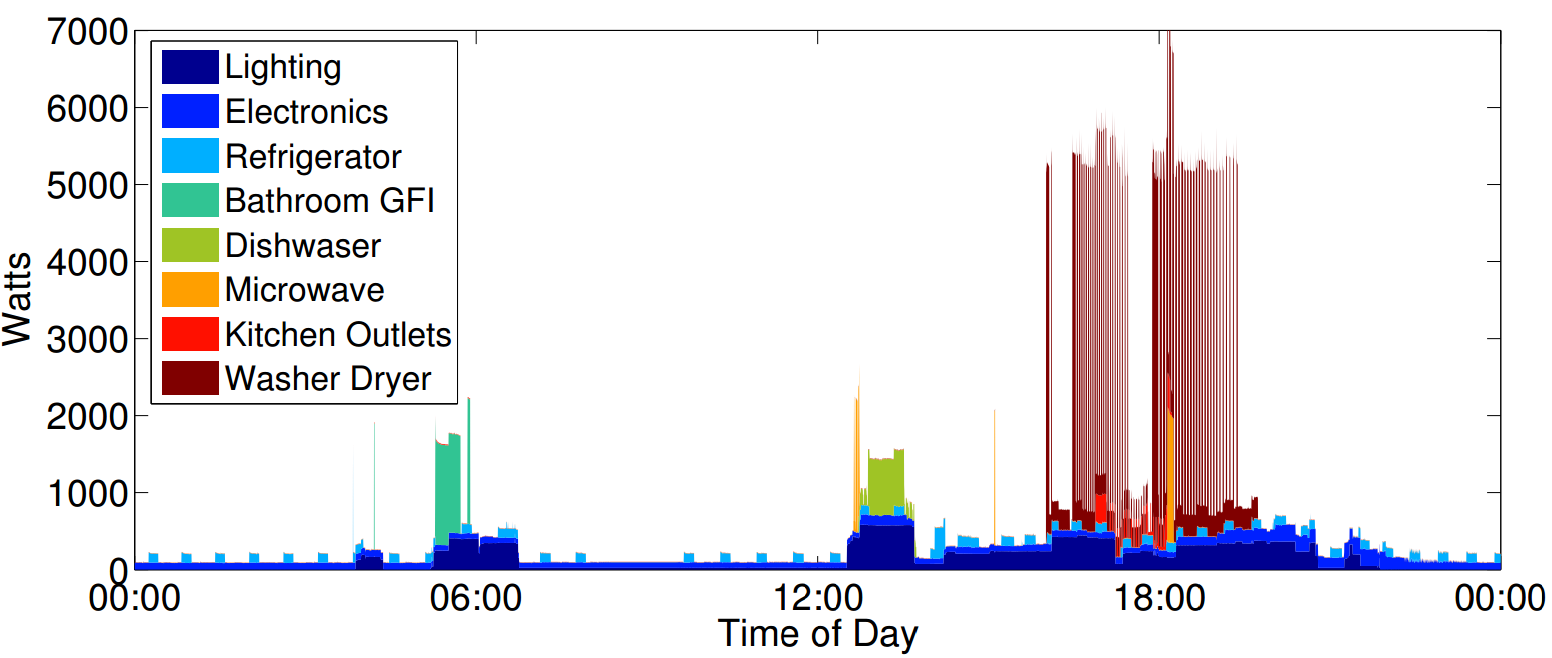
\includegraphics[width=\textwidth]{chapters/introduction-chapters/energy-consumption-house.png}
	\caption{An example of energy consumption of a household over the course of a day \cite{kolter2011redd}.}
	\label{fig:energy-consumption-house}
\end{figure}




If every light in a household has a unique power draw, that is distinguishable from all other lights, the consumer can get better insight in how the lighting is being used in his household. 
With that information, lights that are being used to light a room in the middle of the day for example or in an unoccupied room, can be turned off.
Thereby saving energy and costs.


The unique power draw of each light can be managed through VLC (Visible Light Communication).
With this information that is being sent via VLC, the light can act as a beacon for indoor localization \cite{Kuo:2014:LIP:2639108.2639109}.
For example a smart-phone could then locate itself inside a building with good accuracy.
The ID of the LED beacon which is sent via VLC will also propagate via the current that the LED draws.
The IDs must be chosen in such a way that a smart-meter is still able to identify them on a per lamp basis.
And the current that is drawn must have a shape that can be added with similar patterns so that the smart-meter can make sense of this aggregated current and can start to identify if a LED is on or off.






% !TeX root = ../../thesis.tex


\section{Problem Definition}

Energy disaggregation can detect energy consumers based off the distinct power draw that these devices have.
What it cannot yet do, is the disaggregation of appliances that have very similar power draw, such as lighting.


% !TeX root = ../../thesis.tex


\section{Thesis Contributions}

The aim of this thesis is to propose a framework consisting of theoretical methods, hardware and software, so that lights with similar power draw can be distinguished with a single smart-meter.
This thesis takes advantage of advances in two areas: CDMA codes and VLC.

The specific contributions of this thesis are:

\begin{itemize}

	\item Coding methods are analyzed to allow each LED to have a unique power draw. 
	These codes make it possible to identify if an LED is on or off, even when multiple LEDs are modulating and thereby interfering with each others unique current signature.




	\item Hardware is introduced to allow the LEDs to be modulated by a micro controller. 
	This will allow the LEDs propagate their unique signature via either AC or DC. 
	And there is also hardware introduced that can sample the current that all the LEDs are drawing, via either AC or DC.
	The sampled current is then processed by another separate micro controller, which can then state which LEDs are on and which or off.




	\item An evaluation of the proposed hardware and software is carried out, with a testbed which uses standard LED light fixtures. For larger scale evaluations, software simulation is used. 
\end{itemize}


% maybe more ..

% !TeX root = ../../thesis.tex

\section{Thesis Organization}

The remainder of this thesis is organized as follows.
First the related work and the new proposed method is discussed in \autoref{chp:related-work}.
Then the design requirements are outlined in \autoref{chp:design-requirements}.
In \autoref{chp:cdma} the theory about code sequences is explained.
Next, in \autoref{chp:hardware-design}, the existing hardware and the design of the new hardware is discussed.
In \autoref{chp:evaluation} the hardware and software is evaluated for small scale scenarios and simulations are shown for large scale scenarios.
Finally the work is concluded in \autoref{chp:conclusionsandfuturework} and future work is identified.








